\documentclass[a4paper]{article}

\usepackage[english]{babel}
\usepackage[utf8]{inputenc}
\usepackage{fullpage}
\usepackage{amsmath}
\usepackage{graphicx}
\usepackage[colorinlistoftodos]{todonotes}
\usepackage{hyperref}
\usepackage{amssymb}
\usepackage{outline} \usepackage{pmgraph} \usepackage[normalem]{ulem}
\usepackage{graphicx} \usepackage{verbatim}
% \usepackage{minted} % need `-shell-escape' argument for local compile

\title{
    \textbf{\huge Pathways to Green Growth} \\
    \vspace{1cm}
    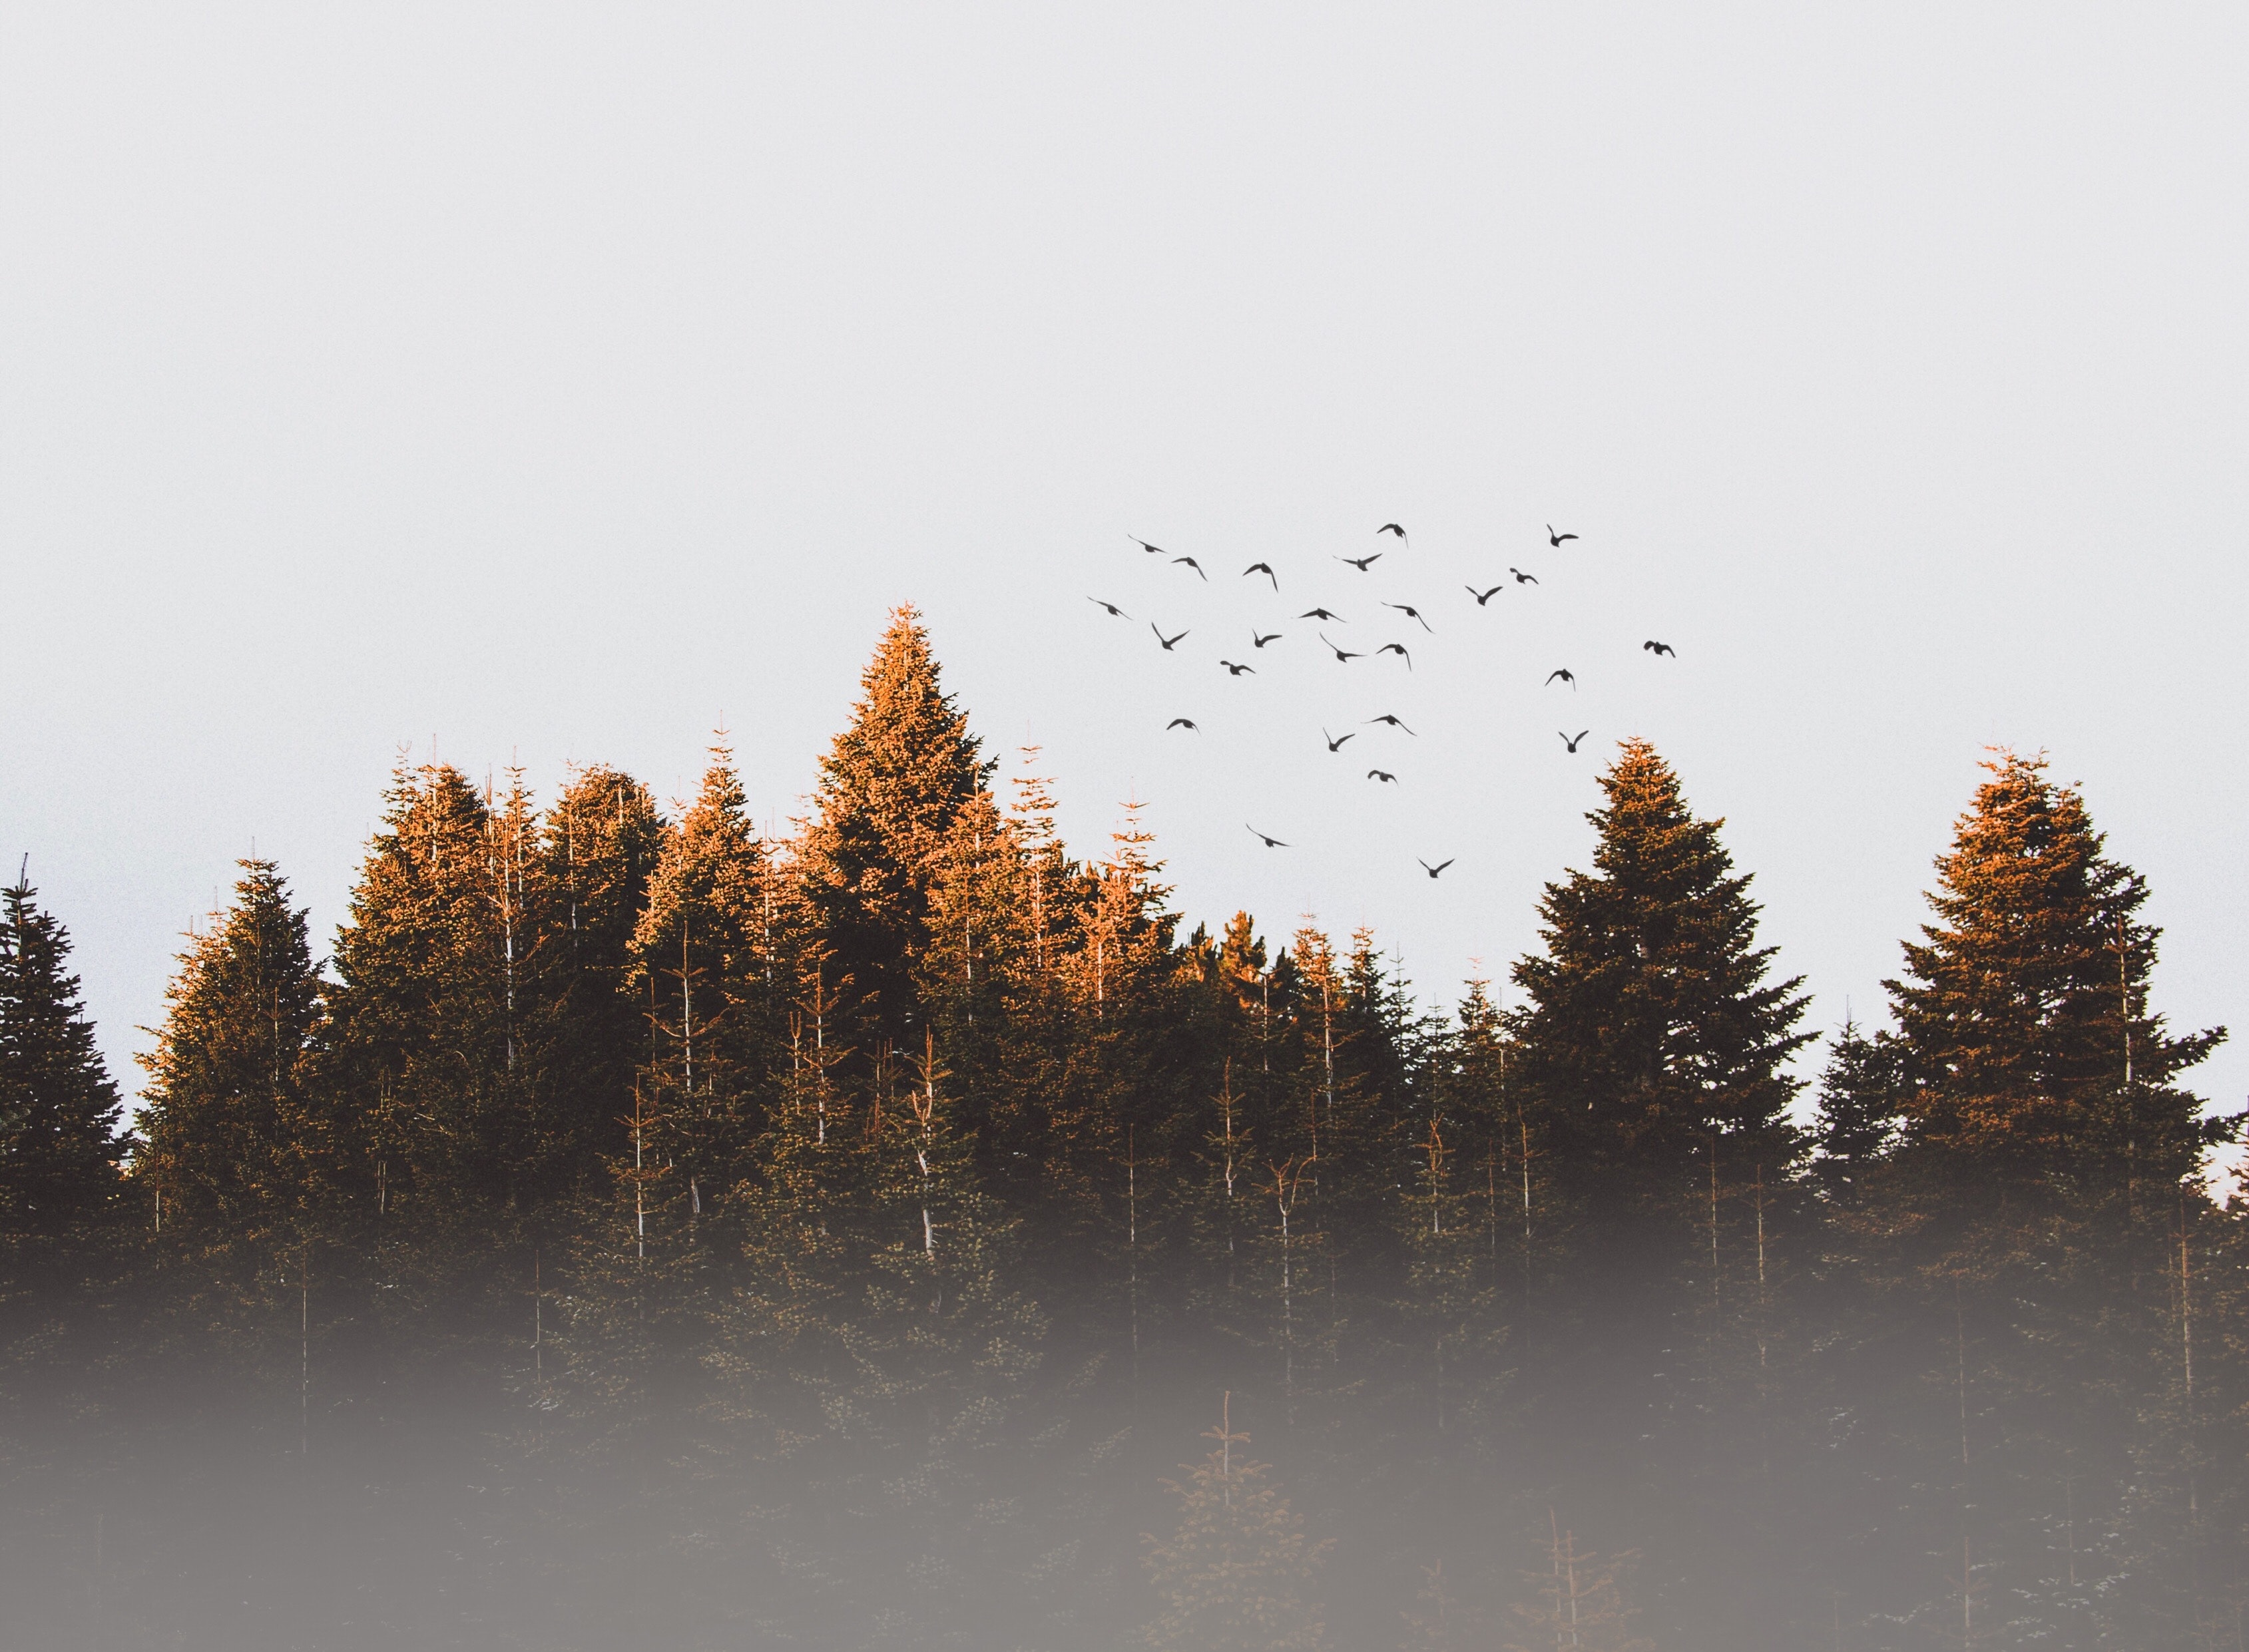
\includegraphics[width=4in]{figures/forest} \\
    \vspace{1cm}
}

\author{\textit{by} \\\\ Can Yilmaz Altinigne \\ Cyril van Schreven \\ Günes Yurdakul \\ \\ \\ \\
    \textbf{\Large EPFL COM-480 Data Visualization: Term Project} \\ \\
    \textbf{Process Book} \\ \\ \\ \\ \\
    
\includegraphics[width=2in]{figures/epfl_logo}\\
}


\begin{document}

\maketitle
\setcounter{page}{0}
\thispagestyle{empty}
\newpage


\section{Introduction}
\large This document is prepared for presenting the development process of an EPFL Data Visualization (COM-480) course project: Map of International Environmental Projects. 
This process book starts with the thought process of the project and continues with revealing the production phase of the project. \\

Data Visualization course aims to provide insights on presenting complex data with interactive visualizations. Our main purpose during the project is to present the 
data with an informative and interactive web application. We benefit from what we learned about chart and map visualization as well as the design process and storytelling with data during the lectures.

\section{Overview}

This project can be thought as a spatial table of contents for the to-be-published book about Green Development and International Experience in Ecosystem Services Management. 
This project aims to locate about 20 case studies across the world. These example are all about ecosystem management (e.g Carbon market, conservation lands, water-funds etc.).

\section{Motivation}

As a team, we were already interested in map visualization because of our experience in this subject in the projects of other courses.
Also, we had some experience in web application development. Since this project brings these two subjects together, we decided to pick this project.
Moreover, the possibility of use of this application as an online supplement for a to-be-published book was another source of motivation for us, since the readers
of this book may benefit from our visualizations to understand the main concepts in the book.

\section{Target Audience}

\section{Related work and inspiration}

\section{Project Implementation}

\subsection{What is visualized in this project ?}
What am I trying to show my viz?

\subsection{Dataset}
where does it come from, what are you processing steps?

\subsection{Data Analysis}
What viz have you used to gain insights on the data?

\subsection{Design}
What are the different visualizations you considered? Justify the design decisions you made using the perceptual and design principles.
Include your sketches, wireframes, etc.

\subsection{Peer assessment}

Preparation – were they prepared during team meetings?

Contribution – did they contribute productively to the team discussion and work?

Respect for others’ ideas – did they encourage others to contribute their ideas?

Flexibility – were they flexible when disagreements occurred?
\vspace{2cm}
\hrule

\section{Research approach}

Write down the approach you use in your research study, this will help you when writing the ``Method'' part in the paper. You may reference some papers like~\cite{isola2017image}.


\section{Research progress}

How much work you have done before this work? Write down your previous work for this project, so people can quickly figure out where you are in your road map now. Yeah, maybe you walked through a long and hard road.

Maybe you have got many data and results, list some necessary here, like Table~\ref{tab:result} shows.

\begin{table}[hb]
    \centering
    \begin{tabular}{c|c}
        \hline \\
        name & value \\
        \hline \\
        a & 0 \\
        \hline \\
        b & 1 \\
        \hline
    \end{tabular}
    \caption{Your experiment result.}
    \label{tab:result}
\end{table}


\section{Progress in this week}

List what you have done in this week in detail.

For example, maybe you performed some experiments this week. The following are the steps you took:

\begin{description}
\item [Step 1]
Got up to welcome a new day.
\item[Step 2]
Opened your computer to start a new day's work.
\item[Step 3]
Got stuck with a very hard problem, like $e^{i \pi} + 1 = 0$.
\item[Step 4]
You searched online and realized some useful information like Figure~\ref{fig:google} shows. You asked other people for help and got the things done luckily.
\end{description}

\begin{figure}[hb]
    \centering
    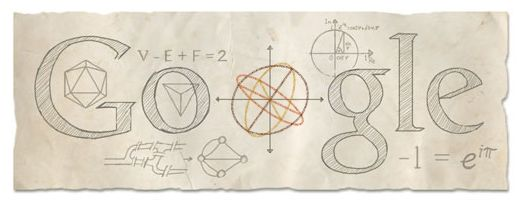
\includegraphics{figures/google}
    \caption{Search online to get some useful information.}
    \label{fig:google}
\end{figure}

But there are still some problems confusing you, then you need to keep calm and carry on.

\section{Plan}

\begin{tabular}{rl}
	\textbf{Objective:} & XXXX \\
    \textbf{Deadline:} & XXXX 
\end{tabular}

\begin{description}
    \item[\normalfont 2018.05.07---2018.05.14] Do something.
    \item[\normalfont 2018.05.15---2018.05.22] Do something else.
    \item[\normalfont 2018.05.23---2018.05.31] Do a lot lot lot lot lot lot lot lot lot lot lot lot of things.
\end{description}

% If you don't cite any references, please comment the following two lines
\bibliographystyle{ieee}
\bibliography{ref.bib}

\end{document}
